\documentclass{article}\usepackage[]{graphicx}\usepackage[]{color}
% maxwidth is the original width if it is less than linewidth
% otherwise use linewidth (to make sure the graphics do not exceed the margin)
\makeatletter
\def\maxwidth{ %
  \ifdim\Gin@nat@width>\linewidth
    \linewidth
  \else
    \Gin@nat@width
  \fi
}
\makeatother

\definecolor{fgcolor}{rgb}{0.345, 0.345, 0.345}
\newcommand{\hlnum}[1]{\textcolor[rgb]{0.686,0.059,0.569}{#1}}%
\newcommand{\hlstr}[1]{\textcolor[rgb]{0.192,0.494,0.8}{#1}}%
\newcommand{\hlcom}[1]{\textcolor[rgb]{0.678,0.584,0.686}{\textit{#1}}}%
\newcommand{\hlopt}[1]{\textcolor[rgb]{0,0,0}{#1}}%
\newcommand{\hlstd}[1]{\textcolor[rgb]{0.345,0.345,0.345}{#1}}%
\newcommand{\hlkwa}[1]{\textcolor[rgb]{0.161,0.373,0.58}{\textbf{#1}}}%
\newcommand{\hlkwb}[1]{\textcolor[rgb]{0.69,0.353,0.396}{#1}}%
\newcommand{\hlkwc}[1]{\textcolor[rgb]{0.333,0.667,0.333}{#1}}%
\newcommand{\hlkwd}[1]{\textcolor[rgb]{0.737,0.353,0.396}{\textbf{#1}}}%
\let\hlipl\hlkwb

\usepackage{framed}
\makeatletter
\newenvironment{kframe}{%
 \def\at@end@of@kframe{}%
 \ifinner\ifhmode%
  \def\at@end@of@kframe{\end{minipage}}%
  \begin{minipage}{\columnwidth}%
 \fi\fi%
 \def\FrameCommand##1{\hskip\@totalleftmargin \hskip-\fboxsep
 \colorbox{shadecolor}{##1}\hskip-\fboxsep
     % There is no \\@totalrightmargin, so:
     \hskip-\linewidth \hskip-\@totalleftmargin \hskip\columnwidth}%
 \MakeFramed {\advance\hsize-\width
   \@totalleftmargin\z@ \linewidth\hsize
   \@setminipage}}%
 {\par\unskip\endMakeFramed%
 \at@end@of@kframe}
\makeatother

\definecolor{shadecolor}{rgb}{.97, .97, .97}
\definecolor{messagecolor}{rgb}{0, 0, 0}
\definecolor{warningcolor}{rgb}{1, 0, 1}
\definecolor{errorcolor}{rgb}{1, 0, 0}
\newenvironment{knitrout}{}{} % an empty environment to be redefined in TeX

\usepackage{alltt}
\usepackage{Sweave}
\usepackage{float}
\usepackage{graphicx}
\usepackage{tabularx}
\usepackage{siunitx}
\usepackage{amssymb} % for math symbols
\usepackage{amsmath} % for aligning equations
\usepackage{textcomp}
\usepackage{mdframed}
\usepackage[T1]{fontenc}
\usepackage{subcaption}
\usepackage{natbib}
\bibliographystyle{..//refs/styles/besjournals.bst}
\usepackage[small]{caption}
\setlength{\captionmargin}{30pt}
\setlength{\abovecaptionskip}{0pt}
\setlength{\belowcaptionskip}{10pt}
\captionsetup{justification=raggedright,singlelinecheck=false}
\topmargin -1.5cm        
\oddsidemargin -0.04cm   
\evensidemargin -0.04cm
\textwidth 16.59cm
\textheight 21.94cm 
%\pagestyle{empty} %comment if want page numbers
\parskip 7.2pt
\renewcommand{\baselinestretch}{1.5}
\parindent 0pt
%\usepackage{lineno}
%\linenumbers

%cross referencing:
\usepackage{xr}
\usepackage{xr-hyper}
\externaldocument{/Users/CatherineChamberlain/Documents/git/microclimates/docs/micro_supp}

\newmdenv[
  topline=true,
  bottomline=true,
  skipabove=\topsep,
  skipbelow=\topsep
]{siderules}
\IfFileExists{upquote.sty}{\usepackage{upquote}}{}
\begin{document}

\noindent\textbf{\Large{Comparing spring phenology in an urban arboretum versus rural forested site and implications for forecasting}}

\noindent Authors:\\
C. J. Chamberlain $^{1,2}$ \& E. M. Wolkovich $^{1,2,3}$
\vspace{2ex}\\
\emph{Author affiliations:}\\
$^{1}$Arnold Arboretum of Harvard University, 1300 Centre Street, Boston, Massachusetts, USA; \\
$^{2}$Organismic \& Evolutionary Biology, Harvard University, 26 Oxford Street, Cambridge, Massachusetts, USA; \\
$^{3}$Forest \& Conservation Sciences, Faculty of Forestry, University of British Columbia, 2424 Main Mall, Vancouver, BC V6T 1Z4\\
\vspace{2ex}
$^*$Corresponding author: 248.953.0189; cchamberlain@g.harvard.edu\\

\renewcommand{\thetable}{\arabic{table}}
\renewcommand{\thefigure}{\arabic{figure}}
\renewcommand{\labelitemi}{$-$}
\setkeys{Gin}{width=0.8\textwidth}

%%%%%%%%%%%%%%%%%%%%%%%%%%%%%%%%%%%%%%%%%%%%%%%
%%%%%%%%%%%%%%%%%%%%%%%%%%%%%%%%%%%%%%%%%%%%%%%


\section*{Introduction}
\begin{enumerate}
\item Understanding and predicting plant phenology in temperate deciduous forests is critical as it both shapes community structure and also influences major ecosystem services such as resource and forest management. 
  \begin{enumerate} 
  \item Climate change and urbanization are advancing spring timing---such as budburst and leafout, which  are strongly cued by temperature, resulting in longer growing seasons \citep{Chuine2001} which ultimately impacts these services.  
  \item   Spring budburst timing can have cascading effects to pollinators \citep{Boggs2012, Pardee2017}, on albedo \citep{Williamson2016}, and on carbon dynamics \citep{Richardson2013} 
  \item Temperate forests sequester carbon and help mitigate the negative effects of climate change and---with earlier spring phenology and longer growing seasons---there has been an increase in carbon uptake \citep{Keenan2014}.
  \item Because of the importance of phenology, forecasting it accurately with climate change is a major and important aim across several fields of science \citep{Moorcroft2001,Taylor2020,Yu2016,Zhao2012}.
  \end{enumerate}
  
\item One major forecasting method across all these fields is the growing degree day model. 
  \begin{enumerate} 
   \item The growing degree day (GDD) model allows researchers to track heat accumulation to measure and forecast spring budburst \citep{Cook2012,Crimmins2020,Phillimore2013,Schwartz2006,Vitasse2011}.
  \item The GDD model simply sums temperatures above a certain threshold---ideally around 0$^{\circ}$C as estimates are proven to be more accurate \citep{Man2010}---and different species often require a different number of GDDs to leaf out. 
  \item GDDs accumulate at a faster rate when mean temperatures are higher, thus different sites or different climate measurement methods may record different GDD thresholds for budburst. 
  \item  Integrating the growing degree day model successfully is essential for predicting the effects of climate change on systems where the climate is rapidly changing, including temperate forests. 
  \end{enumerate}
  
\item We often assume in GDD models, that the GDD required for a species, or even a suite of species (e.g., plant functional types) is constant, but increasing evidence suggests it may not be.
  \begin{enumerate} 
  \item The plasticity of phenology means that the same individual exposed to different climates will leafout at a very different time. Decades of work show that chilling---related to winter temperatures---and photoperiod can shift the GDD a plant needs for the same event \citep{Basler2012,Chuine2010,Zohner2016}.
  \item Spring phenology also has a genetic component, and the required chilling, photoperiod and GDD can vary by population \citep{Scotti2004,Cuervo-Alarcon2018}. Though this effect does seem smaller than for other phenological events \citep{McKown2013,Satake2013}.
  \end{enumerate}

\item Climate helps determine the role of chilling and photoperiod, this could be climate on a larger or smaller scale. 
  \begin{enumerate} 
  \item On a large scale, there are climate gradients across space (i.e., latitudinal or continentality effects), but also gradients due to anthropogenic impact. 
  \item Urbanization has led to the formation of urban heat islands, which have been shown to affect plant phenology and lead to earlier spring leafout \citep{Meng2020}. 
  \item Because urban sites strongly contribute to carbon sequestration \citep{Ziter2018}, these trends are crucial to understand in order to predict plant development with warming. 
  \item Increasingly, researchers have suggested that urban environments  provide a natural laboratory for assessing the effects of warming on temperate tree and shrub species as these sites are warming at a faster rate than more rural habitats \citep{Pickett2011, Grimm2008}.
  \item Additionally urban sites often house arboreta or botanical gardens that often contribute long-term records \citep{Zohner2014} or are used for experiments on phenology \citep{Ettinger2018}.
  \item Arboreta and botanical gardens offer a unique lens to investigate climate change and local adaptation studies by incorporating varying seed sources---or provenance locations---thus they mimic common garden experiments \citep{Primack2009}.   \item Thus understanding if results from such urban sites directly translate to more natural forests is important also. 
  \end{enumerate}
  
\item Climate on a smaller scale may also be important to consider. 
  \begin{enumerate} 
  \item Climate can vary a lot on small spatial scales \citep[][e.g., as much as 2.6$^{\circ}$C between sensors at the same vineyard or up to 6.6$^{\circ}$C within 1 km spatial units in northern Europe]{deResseguier2020,Lenoir2013}.
  \item Thus, increasing evidence suggests that fine-scale climate may matter to phenology \citep{Lembrechts2019}.
  \item Additionally, temperature variation at the bud level is shown to affect budburst timing within an individual canopy \citep{Lembrechts2019}.
  \item To facilitate scaling and minimize error due to these fine-scal climatic effects (i.e., microclimate effects), researchers often deploy standalone weather loggers---such as HOBO sensors---which may provide higher resolution weather data \citep{Schwartz2013a,Whiteman2000}.
  \item Though deploying temperature loggers is not always feasible, especially when investigating large spatiotemporal shifts in GDDs. 
  \end{enumerate}
  
\item Provenance may also matter, though evidence is lacking for spring phenological phases \citep{Aitken2015, McKown2013}.
  \begin{enumerate} 
  \item There is large debate over the role of provenance latitude on budburst initiation and the associated shifts in phenological cue use. 
  \item Some studies suggest that: (1) species from lower latitudes will be more reliant on photoperiod with climate change \citep{Zohner2016}, (2) photoperiod will slow or constrain range expansion \citep{Saikkonen2012}, (3) all species will rely on photoperiod more as winters warm \citep{Way2015}, and (4) lower latitude species will require both strong photoperiod cues and more forcing in order to compensate for the lack of chilling but photosensitivity may be more important at the cold trailing edge for range expansion to occur \citep{Gauzere2017}.
  \item  Many arboreta keep diligent acquisition records, providing visitors and scientists information on seed sources \citep{Dosmann2006}, and the potential to test such provenance effects.
  \end{enumerate}

\item Here we aimed to address the following hypotheses:
  \begin{enumerate} 
  \item Required GDD in an urban arboreta will vary from a rural forested site. We predicted lower chilling in the urban site could lead to greater required GDD.
  \item Microclimates will lead to variation in GDD within sites. 
  \item Individuals with provenance latitudes from more northern locations require fewer GDDs to budburst. 
  \item We tested these in one urban arboreta and one rural forested site and we additionally incorporated simulations to help better interpret our results. 
  \end{enumerate}
\end{enumerate}

\section*{Methods}
\subsection*{Sites}
\begin{enumerate}
\item We chose two sites---one urban arboretum and one forest---with overlapping species and climates to compare the number of growing degree days to budburst across species. 
  \begin{enumerate}
  \item The urban site is in Boston, MA at the Arnold Arboretum of Harvard University (42$^{\circ}$17' N -71$^{\circ}$8' W).
  \item The Arnold Arboretum is 281 acres, contains 3825 woody plant taxa from North America, Europe and Asia and has an elevation gain of approximately 96m.
  \item The forest site is in Petersham, MA at the Harvard Forest (42$^{\circ}$31'53.5' N -72$^{\circ}$11'24.1' W).
  \item The Harvard Forest is 1446 acres and has a range of elevation of 220-410m. 
  \end{enumerate}
\end{enumerate}
  

\subsection*{Simulations}
\begin{enumerate}
\item We simulate test data in order to assess our model output results, especially our inference on teasing out effects of microclimates versus provenance versus potential differences across weather station and hobo logger data. Our sims were designed to test the following potential effects:
  \begin{enumerate}
  \item (1) urban environments require more GDDs,
  \item (2) presence of microclimates (at one or both sites) accurately measured by hobo loggers,
  \item (3) presence of provenance effects (i.e., there were multiple provenance latitudes at the urban arboretum site but only one at the rural forest site),
  \item (4) weather stations or hobo loggers are effectively `noisier' data for GDD models compared to the other. 
  \end{enumerate}

\item Our methods for this are broadly as follows:
  \begin{enumerate}
  \item We assume each species needs a different GDD (drawing each species' requirement from a normal distribution).
  \item We model climate data by again establishing a random distribution around a mean temperature for each site. 
 \item Using this climate data, we then find the day of budburst when the unique GDD threshold is reached for each individual. 
  \item To test that urban sites require more GDD, we create simulation data that manipulates the GDD threshold for the urban versus rural sites by increasing the GDD threshold for individuals at the more urban locations (e.g., local arboreta). 
  \item  To test microclimate effects, we build our climate data then add variation to this weather data to create ``microclimate'' effects. 
  \item To test the provenance latitude hypothesis we make individuals from more northern provenances require fewer GDDs.
  \item To test for the effect of noise, we add noise by increasing the sigma value for our random distribution around a mean temperature for each method.
  \end{enumerate}

\item We additionally examined the accuracy of GDD models using different base temperatures and with warming through simulations.
\begin{enumerate}
  \item To evaluate the accuracy of GDD models, we used different base temperatures for calculating GDD (i.e., 0$^{\circ}$C versus 10$^{\circ}$C) with variation in sigma around base temperatures (i.e., 0$^{\circ}$C and 0.5$^{\circ}$C).
  \item We also tested GDD accuracy across various GDD threshold requirements with warming of 1$^{\circ}$C to 10$^{\circ}$C. 
  \item Accuracy was evaluated as a ratio of observed GDD divided by the expected GDD.
\end{enumerate}
\end{enumerate}

\subsection*{Data analysis}
\begin{enumerate}
\item Using Bayesian hierarchical models with the rstan package \citep{rstan2019}, version 2.19.2,  in R \citep{R}, version 3.3.1, we estimated the effects of urban or provenance effect and method effect and all two-way interactions as predictors on GDDs until budburst. 
  \begin{enumerate} 
  \item Species were modeled hierarchically as grouping factors, which generates an estimate and posterior distribution of the overall response across the 15 species used in our simulations and 18 species used in our real data.
  \item We ran four chains, each with 2 500 warm-up iterations and 3 000 iterations for a total of 2 000 posterior samples for each predictor for each model using weakly informative priors.
  \item Increasing priors three-fold did not impact our results.
  \item We evaluated our model performance based on $\hat{R}$ values that were close to one and did not include models with divergent transitions in our results. 
  \item We also evaluated high $n_{eff}$ (3000 for most parameters, but as low as 708 for a couple of parameters in the simulated provenance latitude model). 
  \item We additionally assessed chain convergence and posterior predictive checks visually \citep{BDA}.
  \item We report means $\pm$ 50\% uncertainty intervals from our models in the main text because these intervals are more computationally stable \citep{Carpenter2017,BDA}. See Tables \ref{tab:urban}- \ref{tab:provreal} for 95\% uncertainty intervals. 
  \end{enumerate}
\end{enumerate}

\subsection*{Shiny App}
\begin{enumerate}
\item To show the above simulations, real data and forecasts in one location we use a Shiny Application. 
  \begin{enumerate}
  \item Using the R package `shiny' \citep{shiny2021}, version 1.6.0, we developed a Shiny App that contains five pages: (1) `Home' which has information on the application, (2) `Hypothesis Testing' which runs the simulation data and allows users to manipulate the inputs, (3) `Simulation Data for Model Testing' which runs simulation data to test the model and make sure the model outputs are accurate, (4) `Real Data and Analyze Results' which uses real data and runs analyses to be used to compare to the `Hypothesis Testing' output and (5) `Forecasting GDD with Warming' which forecasts GDD accuracy under warming. 
  \end{enumerate}
\end{enumerate}

\section*{Results}
\subsection*{Simulations -- part 1}
\begin{enumerate}
  \item We find we can accurately recover a simple effect of urban sites requiring more GDD (20.67 $\pm$ 1.17; Figure \ref{fig:musims} \textbf{a)} and Table \ref{tab:urban}).
  \item Simulations that include microclimates at both sites show that the hobo loggers require more GDDs until budburst. 
  \item When simulating microclimate effects---thus greater variation in GDD---across the sites, we include greater variation in temperature for the hobo logger data, which is being reflected by the negative slope of the method parameter (-6.78 $\pm$ 2.57; Figure \ref{fig:musims} \textbf{b)} and Table \ref{tab:micros}). 
  \item Provenance effect simulations indicate more northern provenance locations require fewer GDDs until budburst which is being recovered in the provenance parameter (-4.8 $\pm$ 1.16; Figure \ref{fig:musims} \textbf{c)} and Table \ref{tab:prov}).
  \item When we manipulate the simulations to have noisy weather station data, noise is returned as the sigma for the method parameter (Figure \ref{fig:noisymus} \textbf{a)}) and the method parameter is slightly positive (4.93 $\pm$ 5.25), indicating weather stations require more GDDs until budburst. 
  \item Though, when we manipulate the simulations to have noisy hobo logger data, the output is nearly identical (Figure \ref{fig:noisymus} \textbf{b)}) but the method parameter is slightly negative (-6.41 $\pm$ 5.47), now indicating hobo loggers require more GDDs until budburst.
  \end{enumerate}
  
  \subsection*{Simulations -- part 1 --  GDD accuracy}
\begin{enumerate}
\item The GDD model is most accurate for individuals that have high GDD thresholds and when base temperatures are higher (i.e., 10$^{\circ}$C; Figure \ref{fig:forecasts}). 
  \begin{enumerate}
  \item However, the GDD model becomes less accurate with warming, and accuracy decreases at a faster rate with the higher base temperature (i.e., 10$^{\circ}$C) than with the lower base temperature (i.e., 0$^{\circ}$C; Figure \ref{fig:warming}).
  \item Under the no warming simulation, using the 10$^{\circ}$C base temperature is most consistent across species but with any amount of warming, the 0$^{\circ}$C base temperature is more accurate. 
  \item Additionally, variability in accuracy across GDD thresholds and with warming increases with higher sigmas (Figure \ref{fig:forecasts} and Figure \ref{fig:warming}).
  \end{enumerate}
\end{enumerate}
\end{enumerate}

\subsection*{Real data}
\begin{enumerate}
\item Mean spring temperature at the urban arboretum site was 4.39$^{\circ}$C and was 1.42$^{\circ}$C at the rural forested site using weather station climate data (Figure \ref{fig:clim} \textbf{a)} and \textbf{b)}). 
  \begin{enumerate}
  \item When climate data was recorded with the hobo loggers, mean spring temperature at the urban arboretum was 6.13 and was 1.78$^{\circ}$C at the rural forested site (Figure \ref{fig:clim} \textbf{a)} and \textbf{b)}). 
  \item Overall, the hobo loggers generally recorded higher temperatures than the weather station at the urban arboretum site (with a mean of 1.75$^{\circ}$C and a standard deviation of 1.03$^{\circ}$C; Figure \ref{fig:clim} \textbf{c)} and \textbf{d)}).
  \item The maximum difference between the hobo logger and weather station was 6.34$^{\circ}$C and one logger recorded 2.92$^{\circ}$C higher temperatures on average than the weather station, both of which were at the urban arboretum. 
  \item The rural forested sight generally had more variation around the weather station, though did not typically record higher or lower temperatures than the weather station: the mean difference was 0.55$^{\circ}$C with a standard deviation of 1.04$^{\circ}$C (Figure \ref{fig:clim} \textbf{c)} and \textbf{d)}).
  \item The minimum difference between the hobo logger and weather station was -4.24$^{\circ}$C, which was at the rural forested site and one logger recorded 2.92$^{\circ}$C lower temperatures on average than the weather station at the rural forested site as well. 
  \end{enumerate}

\item Individuals at the arboretum (i.e., more urban sites) require more GDDs to budburst (-31.66 $\pm$ 15.89).
  \begin{enumerate}
  \item There is high variation in GDDs between the two methods (17.09) though the slope is close to zero (method.real $\pm$ method.real.sd).
  \item There is a large interaction indicating weather station data at the arboretum records the fewest number of GDDs until budburst (-40.35 $\pm$ 15.61). 
  \item Using raw data, we see there is higher variation at the arboretum across the two methods and that the arboretum requires fewer GDDs until budburst than the Harvard Forest (i.e., more rural forest sites; Figure \ref{fig:interaction}).
  \end{enumerate}

\item When testing for provenance effects, there was no overall effect of provenance latitude on GDDs until budburst and there was high variation (18.15 $\pm$ 12.96).
  \begin{enumerate}
  \item There was still little effect of method on GDDs until budburst and large variation (-8.46 $\pm$ 8.24).
  \item The interaction of provenance by method was close to zero (-3.53 $\pm$ 12.38) but the sigma was large (13.69).
\end{enumerate}
\end{enumerate}

\section*{Discussion} 
% Below are a few bits from intro that may or may not fit in your discussion
% \item Phenology is often measured through satellite, remote sensing or PhenoCam images to detect spring `green-up' \citep{Meng2020, Liu2018, Richardson2015} but these methods fail to detect the species---or even site-level---nuances in budburst timing \citep{Elmendorf2019}.

\begin{enumerate} 
\item Our study assessed the effects of an urban arboretum versus a more rural forested site coupled with the effect of using weather station versus hobo logger temperature data on GDD until budburst.
  \begin{enumerate} 
  \item We found the urban site was in fact warmer, but this did not translate to individuals requiring more GDDs but rather fewer GDDs until budburst.
  \item Our results additionally suggest there was a strong microclimate effect as is apparent by the large variation in GDD with method.
  \item Though these effects varied by site, with hobo loggers at the urban arboretum generally recording higher temperatures than the weather station but with hobo loggers at the rural forested site recording more variation in temperatures than the associated weather station.
  \item Provenance did not determine clear results so we suggest teasing out provenance effects, given that they may not contribute much to spring phenology \citep{Gauzere2017} and it is difficult with our paucity of latitudinal variation and low sample size for various provenances. 
  \end{enumerate}
  \end{enumerate}

\subsection*{Variation across and within sites suggests important variation for forecasting} 
  \begin{enumerate} 
\item Our finding that urban trees require fewer GDDs contributes to increasing evidence that trees in urban sites may respond differently than those in forested rural areas.
  \begin{enumerate} 
  \item This means that long-term records and experiments conducted in arboreta in urban areas may not be transferrable to larger scale studies and models that incorporate forested rural areas. We should perhaps be more cautious in these extrapolations. 
  \item Our results are in line with other recent studies investigating rural versus urban sites with a lower GDD requirement at urban sites and thus a lower temperature sensitivity \citep{Meng2020} at these sites, with colder rural sites requiring even more GDDs until budburst than their associated urban site.
  \item The lower GDD requirement until budburst is likely due to the arboretum accumulating more over-winter chilling, however, our results become more similar when we use the hobo loggers to measure GDD. 
  \item Recent research suggests individuals can accumulate chilling at temperatures as high as 10$^{\circ}$C \citep{Baumgarten2021}---or even up to 15$^{\circ}$C in subtropical trees \citep{Zhang2021}---but the duration of winter is more important than the temperature. 
  \item If average temperatures are below the chilling accumulation threshold, which may occur at cooler sites, then we can expect less over-winter chilling accumulation at colder sites.
  \item These results suggests we use caution when using urban sites as natural experiments as these sites may not mirror forest habitats, especially when sites are from colder (e.g., more northern) regions.
  \end{enumerate}
  
\item There were no consistent differences in GDDs estimated between the weather stations versus the hobo loggers, but there was a large interaction, which could suggest large, opposing microclimatic differences across the two sites.
  \begin{enumerate} 
  \item The interactive effect was the strongest predictor of GDDs, even stronger than the effect of site.
  \item By disentangling the recorded temperatures between the two methods across the two sites, we see that there is greater variation in hobo logger temperatures at the urban arboretum and these temperatures are generally recording higher temperatures than the weather station.
  \item Whereas at the rural forested site, we see that there is indeed greater variation in temperatures recorded from the hobo loggers than the weather station but that variation is lower than at the urban arboretum and the hobo loggers are recording lower temperatures than the weather station.
  \item As climate is one of the strongest environmental factors contributing to ecosystem change, it is essential to measure weather data as accurately and efficiently as possible, using methods that are accessible to myriad researchers.
  \item And since GDDs are predominant indicators of spring phenology, having accurate and consistent weather data is essential for better estimates of budburst or leafout, especially with warming.
  \item By incorporating both hobo logger and weather station data, we are able to determine microclimate effects across the two sites and detect nuances in canopy temperature variation across two different types of sites: generally open-canopy, urban arboretum versus a typically closed-canopy, rural forest.
  \item The urban arboretum weather station tends to record cooler temperatures than most of the hobo loggers (Figure \ref{fig:clim}) and since these differences in temperature occur close to 0$^{\circ}$C, these differences could in fact be biologically meaningful to phenology. 
  \item In contrast, the climate data from the hobo logger and the weather station seem more similar at the rural forested site.
  \item Given these results, we may see a stronger microclimate effect at the urban arboretum than the rural forested site---which could be true given different tree species create different under canopy effects, or there are more sidewalks and roads, etc.---though more work is necessary to be certain.
  \end{enumerate}
\end{enumerate}

\subsection*{Accurately attributing observed variation requires more research on climate methods and phenology} 
  \begin{enumerate} 
% EMW -- I think we need to give just a few simple messages here!
\item Our simulations suggest teasing out noise versus microclimate effects could be difficult.
  \begin{enumerate} 
  \item As is evident from the model outputs, the method which is less accurate requires more GDDs until budburst since GDDs are accumulating at a faster rate with higher temperature variability---and higher temperature days.
  \item By including microclimate effects at both sites, variation in temperature increases and, thus, the number of days in which the temperature falls below the base GDD threshold is also greater but the days in which temperatures are accumulating, the temperature will likely be greater than what is recorded at the weather station.
  \item High temperature variability, whether it is due to inaccurate recordings or due to microclimates, results in more days at higher temperatures so the day of budburst records higher GDDs for the method with greater temperature variability. 
  \item As climate is one of the strongest environmental factors contributing to ecosystem change, it is essential to measure weather data as accurately and efficiently as possible, while using methods that are accessible to myriad researchers.
  \item Determining which methods are most accurate is the first step to determining fine-scale climatic variation and, ultimately, better forecast phenology under climate change. 
  \end{enumerate}
  
\item Future studies that investigate local climate and phenology are essential and here suggest several pathways to more accurately model GDDs under climate change.
    \begin{enumerate} 
    \item In the field studies, we suggest the implementation of more intensive climate method research including specific studies of hobo loggers and the effects of radiation shields and location in the canopy and to apply these treatments next to weather stations and next to the trees or shrubs of interest. 
    \item We also suggest Increasing studies of how bud temperature matters to budburst and leafout, especially studies that tease out radiative heating effects.
    \item And finally, we propose the use of better models as we found the use of just GDD values may not be as good as models that incorporate the entire GDD model itself (i.e., building from climate data to a thermal threshold within the model).
  \end{enumerate}
  
  \item What our results mean for forecasting today ... As we see from our forecasting simulations, regardless of base temperature threshold, GDD models may not be appropriate for the future with warming \citep{Man2010}. 
  \begin{enumerate} 
    \item This is because with warming, GDDs will accumulate at a faster rate, which will reduce accuracy of determining that actual threshold for budburst phenology. 
  \item Generally higher GDD thresholds means lower a lower GDD observed to GDD expected ratio; this is because being off by a day is a small effect for higher GDD threshold species (and hence greater days) than for lower GDD threshold species, but it really depends on climate variability because high variability means some days you can get accumulate GDDs quickly and that can override the GDD threshold trends. 
  \item In reality temperature variance likely changes over the spring so this is pretty tricky! 
  \item In the future, we need to either use a method that is less reliant on accumulated sums---especially if it is a climatilogical sum---or we must scrutinize results through the use of mixed models and simulated data as we demonstrate here.
  \end{enumerate}
\end{enumerate}



\bibliography{..//refs/micro}

\section*{Tables and Figures}

{\begin{figure} [H]
  \begin{center}
  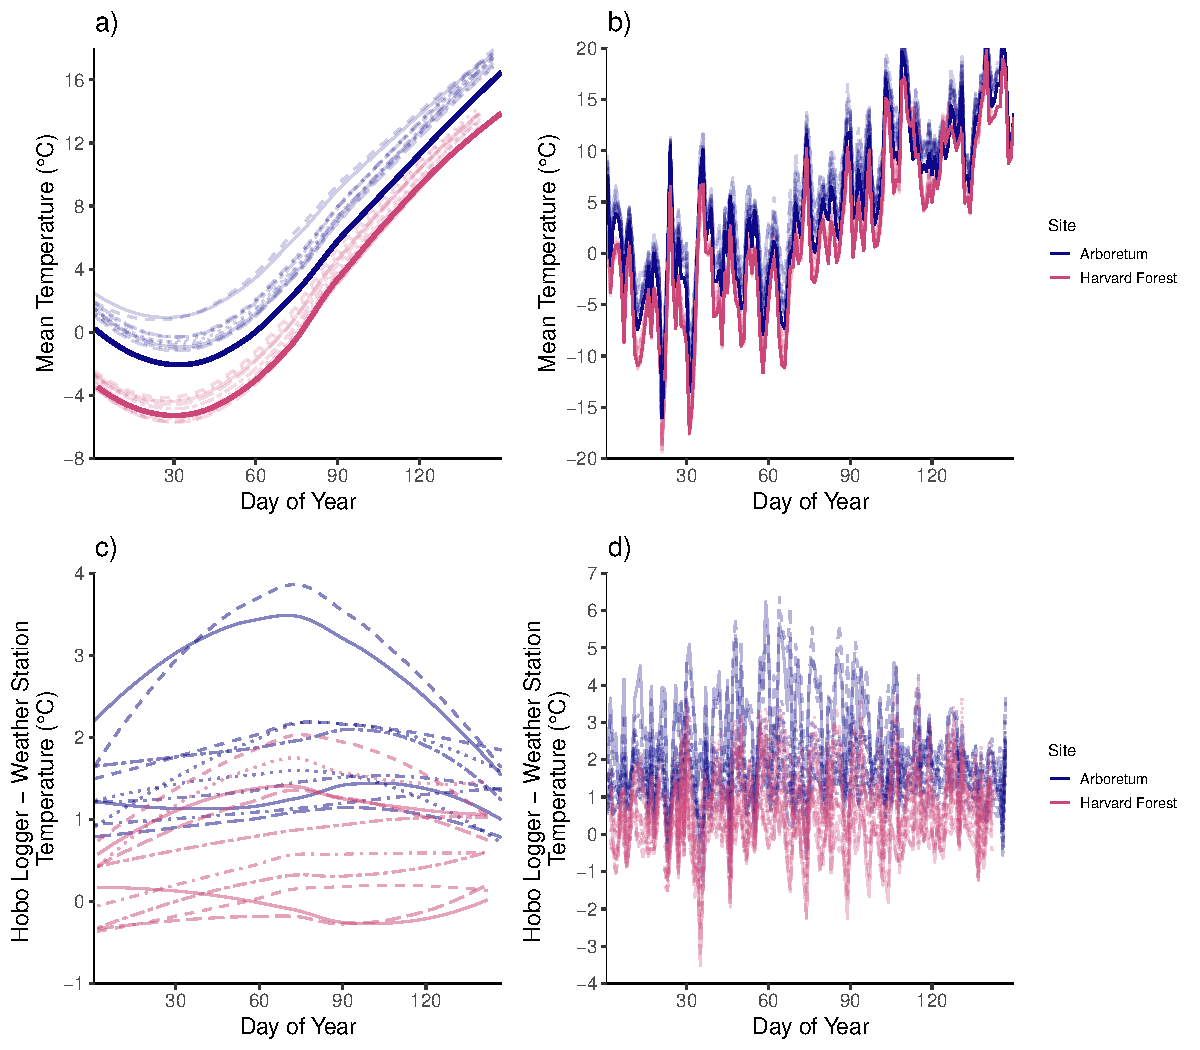
\includegraphics[width=16cm]{..//analyses/figures/clim_4panel.pdf}
  \caption{Here we show a breakdown of the climate data across the two sites with darker lines representing weather station data and the lighter, more transparent lines of varying line types representing the hobo loggers: a) a series of smoothing splines of mean temperature with 90\% credible interval; b) actual mean temperature; c) a series of smoothing splines of mean temperature differences measured as hobo logger minus weather station; and d) actual mean temperature differences measured as hobo logger minus weather station.}\label{fig:clim}
  \end{center}
  \end{figure}}
  
  
\begin{figure}[H]
  \begin{subfigure}{.33\linewidth}
	  %\rule{\linewidth}{\dimexpr 2\linewidth+2\baselineskip+6pt}
    \caption{}
      \centering
      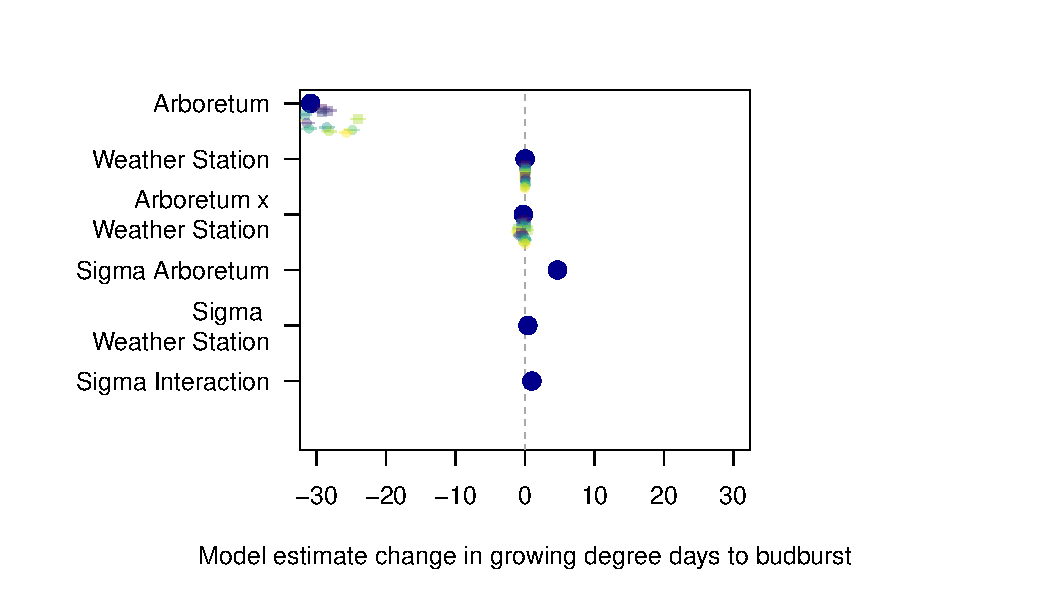
\includegraphics[height=4cm, width=7cm]{..//analyses/figures/muplot_urban.pdf}
      \label{fig:muurban}
  \end{subfigure}%
    \begin{subfigure}{.33\linewidth}
	    %\rule{\linewidth}{\linewidth}
      \caption{}
      \centering
      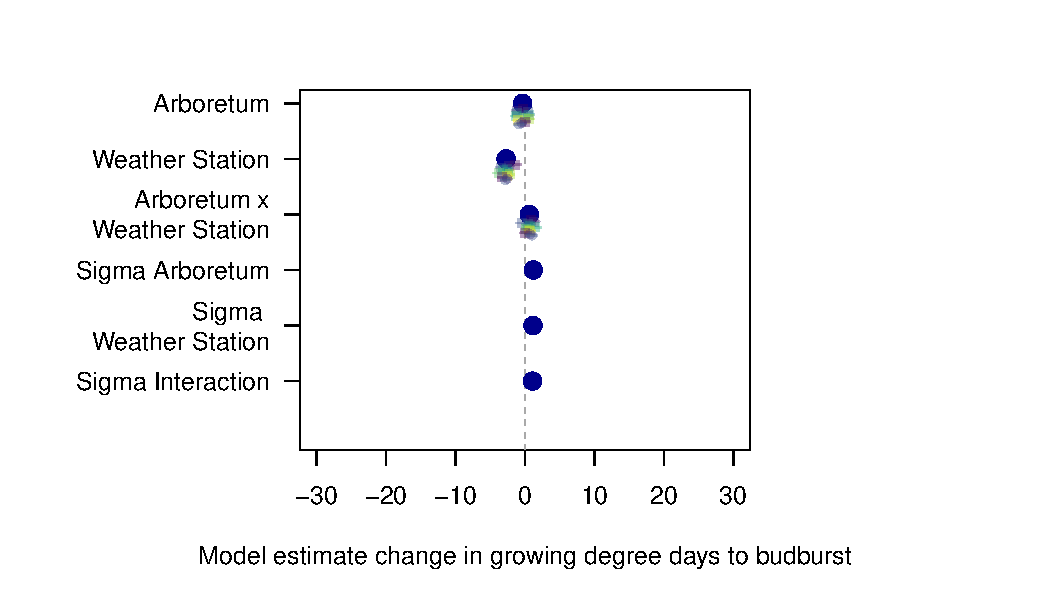
\includegraphics[height=4cm, width=7cm]{..//analyses/figures/muplot_micros.pdf}
    \label{fig:mumicros}
  \end{subfigure}
  \begin{subfigure}{.33\linewidth}
	    %\rule{\linewidth}{\linewidth}
      \caption{}
      \centering
      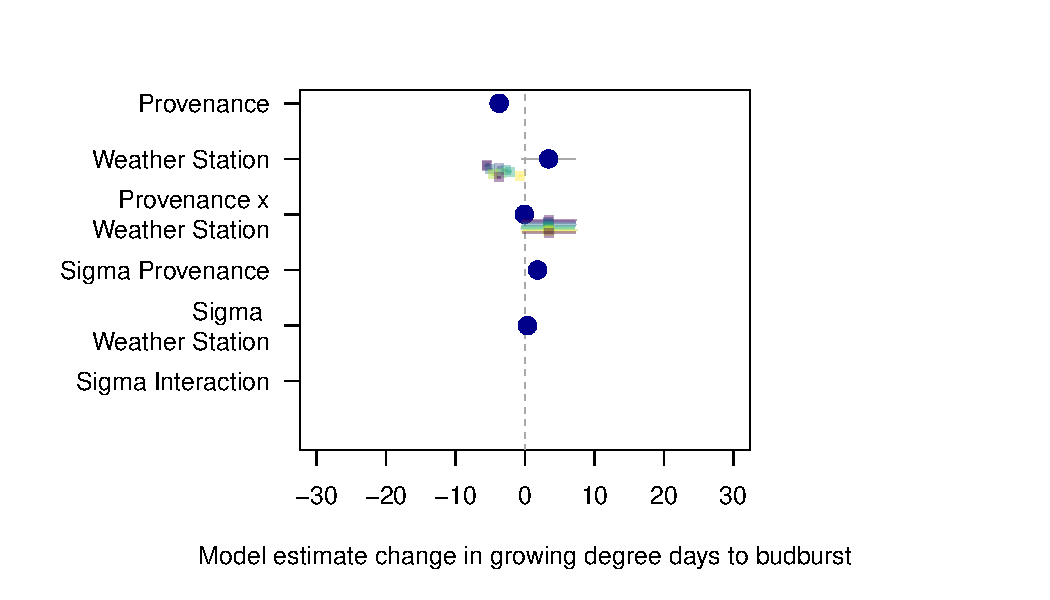
\includegraphics[height=4cm, width=7cm]{..//analyses/figures/muplot_prov.pdf}
    \label{fig:muprov}
  \end{subfigure}
\caption{ Using simulations (a) urban sites requiring more GDDs, (b) microclimate effects and (c) more northern provenance latitudes requiring fewer GDDs, we show the effects of site (urban site is `1' and rural site is `0') and climate data method (weather station data as `1' or hobo logger data as `0') on simulated growing degree days (GDDs) until budburst using. More positive values indicate more GDDs are required for budburst whereas more negative values suggest fewer GDDs are required. Dots and thin lines show means and 90\% uncertainty intervals and thick lines show 50\% uncertainty intervals. See Tables \ref{tab:urban}, \ref{tab:micros} and \ref{tab:prov} for full model output. }
\label{fig:musims}
\end{figure}
  
\begin{figure}[H]
  \begin{subfigure}{.5\textwidth}
	  %\rule{\linewidth}{\dimexpr 2\linewidth+2\baselineskip+6pt}
    \caption{}
    \centering
    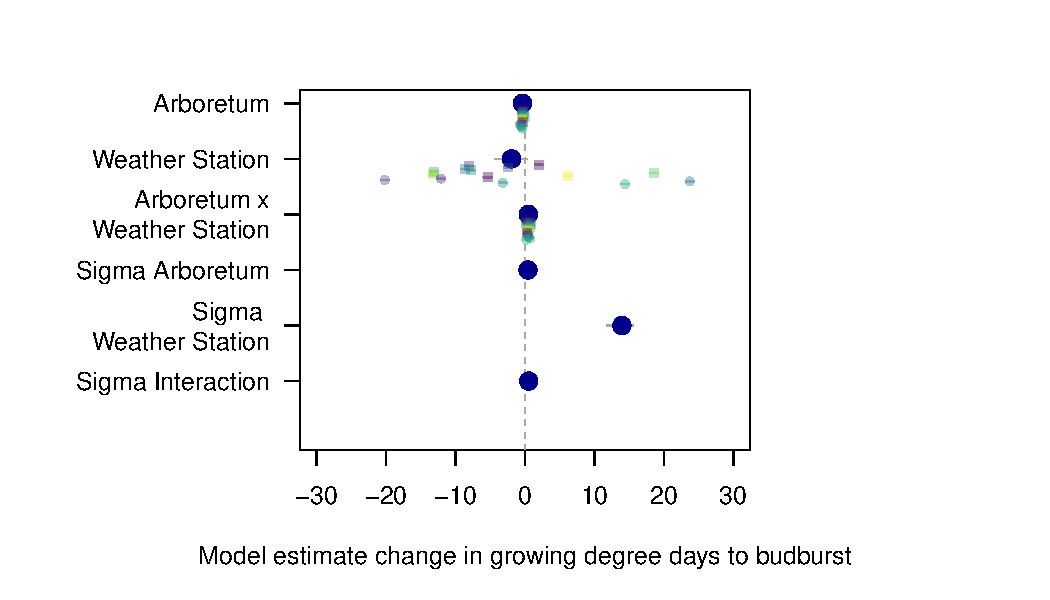
\includegraphics[height=6cm, width=10cm]{..//analyses/figures/muplot_noisyws.pdf}
    \label{fig:muplotnoisyws}
  \end{subfigure}%
    \begin{subfigure}{.5\textwidth}
	    %\rule{\linewidth}{\linewidth}
      \caption{}
      \centering
      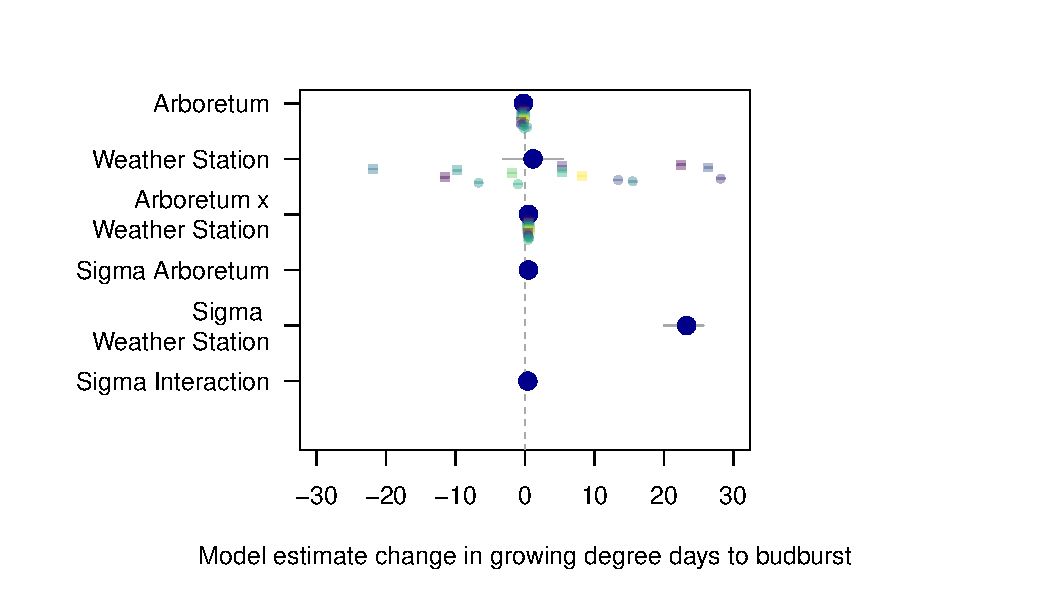
\includegraphics[height=6cm, width=10cm]{..//analyses/figures/muplot_noisyhobo.pdf}
    \label{fig:muplotnoisyhobo}
  \end{subfigure}
\caption{ We show effects of site (urban site as `1' or rural site as `0') and climate data method (weather station data as `1' or hobo logger data as `0') on simulated growing degree days (GDDs) until budburst using simulated data (a) with less accurate weather station data and (b) with less accurate hobo logger data. More positive values indicate more GDDs are required for budburst whereas more negative values suggest fewer GDDs are required. Dots and lines show means and 90\% uncertainty intervals and thick lines show 50\% uncertainty intervals. See Tables \ref{tab:noisyws} and \ref{tab:noisyhobo} for full model outputs.}
\label{fig:noisymus}
\end{figure}


\begin{figure}[H]
  \begin{subfigure}{.5\linewidth}
	  %\rule{\linewidth}{\dimexpr 2\linewidth+2\baselineskip+6pt}
    \caption{}
    \centering
    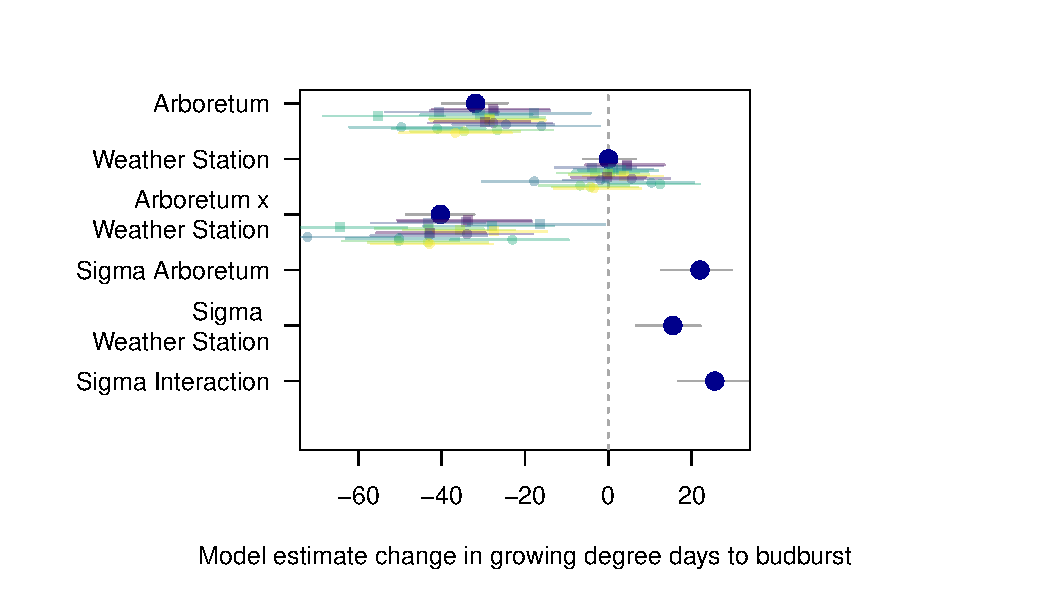
\includegraphics[height=7cm, width=11cm]{..//analyses/figures/muplot_urban_real.pdf}
    \label{fig:muplotreal}
  \end{subfigure}%
    \begin{subfigure}{.5\linewidth}
	    %\rule{\linewidth}{\linewidth}
      \caption{}
      \centering
      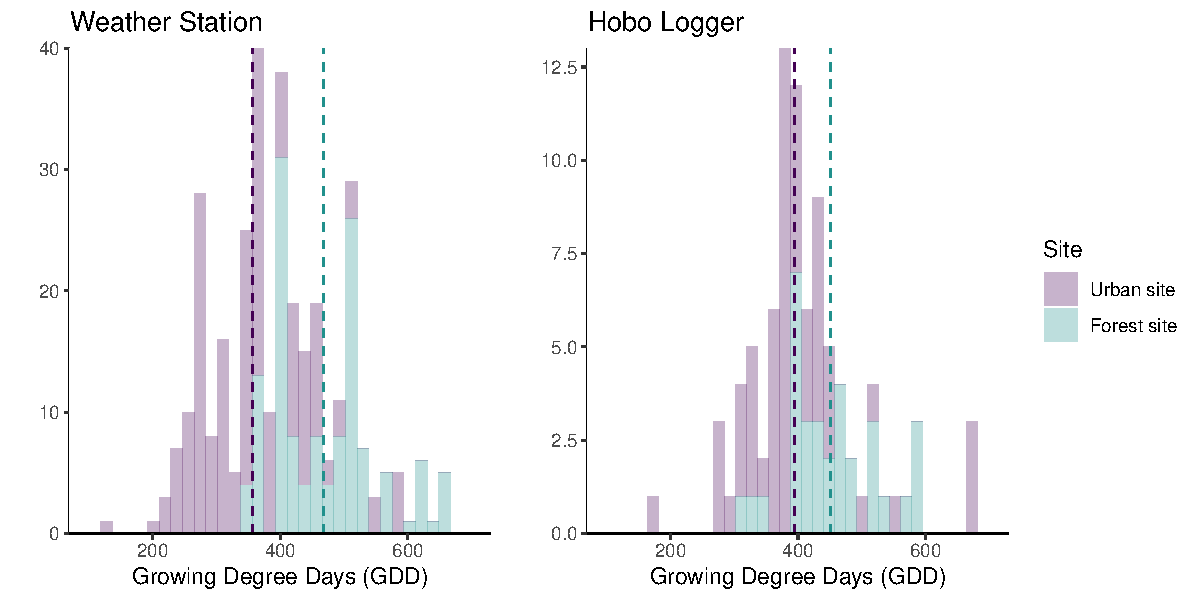
\includegraphics[height=4cm, width=8cm]{..//analyses/figures/gdd_methods_real.pdf}
    \label{fig:gddreal}
  \end{subfigure}
\caption{ Using real data, we show (a) the effects of site (Arboretum is `1' and Harvard Forest is `0') and climate data method (weather station data as `1' or hobo logger data as `0') on simulated growing degree days (GDDs) until budburst using noisy weather station data. More positive values indicate more GDDs are required for budburst whereas more negative values suggest fewer GDDs are required. Dots and thin lines show means and 90\% uncertainty intervals and thick lines show 50\% uncertainty intervals. See Table \ref{tab:real} for full model output. We also show (b) histograms of GDDs at the Arboretum and Harvard Forest using weather station data and hobo logger data.}
\label{fig:real}
\end{figure}

\begin{figure}[H]
      \centering
      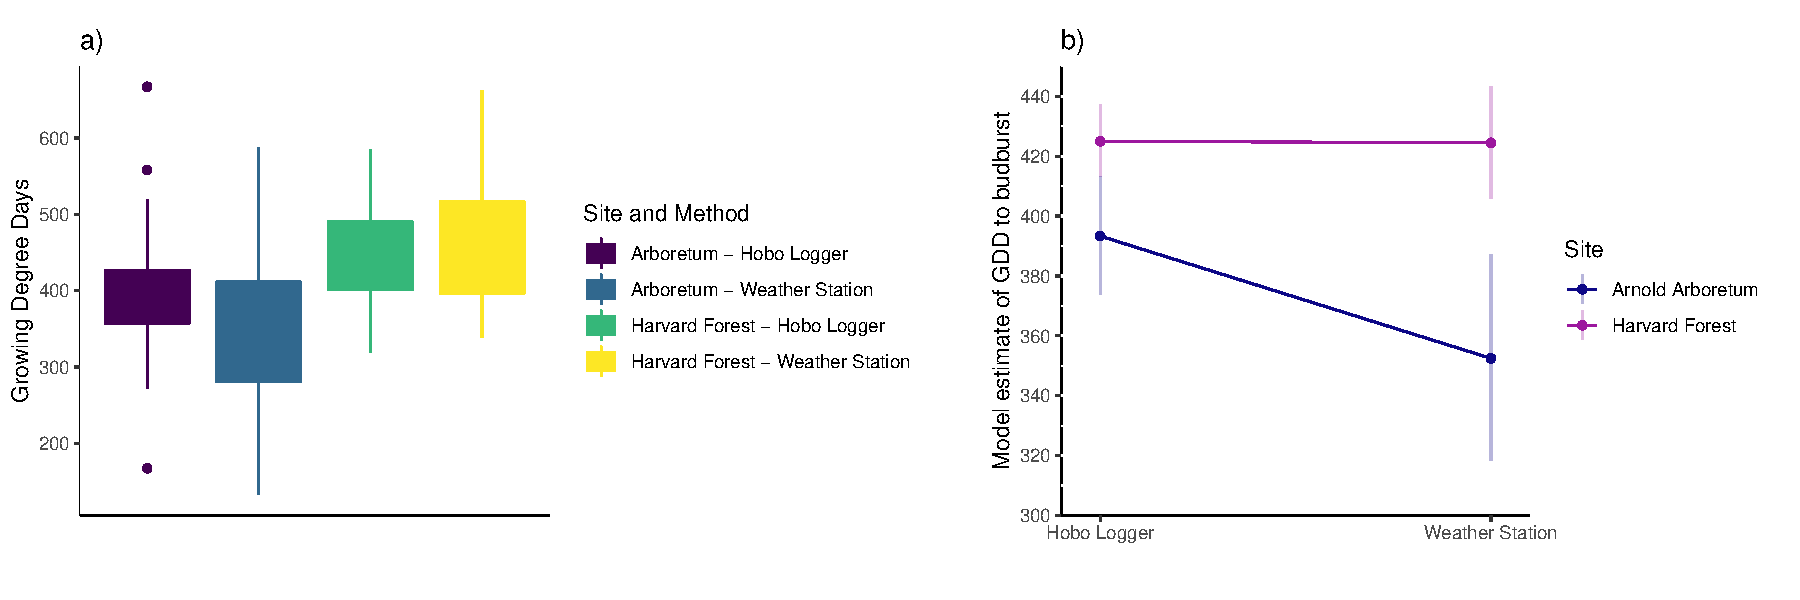
\includegraphics[width=16cm]{..//analyses/figures/gdd_interaction.pdf}
\caption{ We show effects of site (urban arboretum site versus forested rural site) by climate data method (weather station data versus hobo logger data) on growing degree days (GDDs) until budburst (a) as a boxplot across each method and site combination using raw data and (b) using model output to show the mean estimates for each site and method with 50\% uncertainty intervals shown as errorbars.}
\label{fig:interaction}
\end{figure}


\begin{figure}[H]
    \centering
    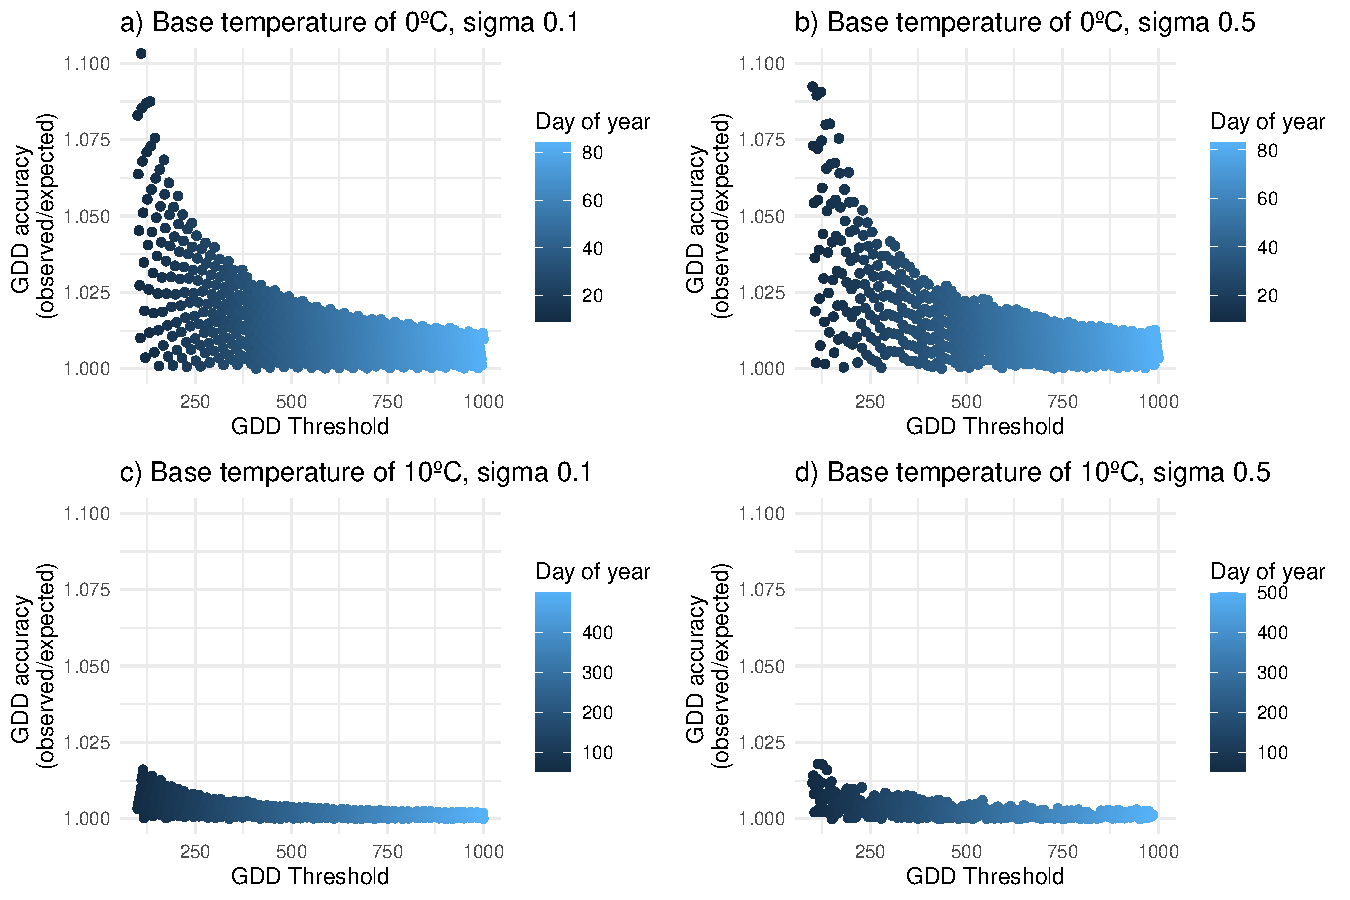
\includegraphics[height=8cm, width=12cm]{..//analyses/figures/gddratio_fstars.pdf}
\caption{Using simulated data, we show how GDD measurement accuracy changes along varying GDD thresholds using a base temperature of (a) 0$^{\circ}$C and a sigma of 0$^{\circ}$C, (b) 0$^{\circ}$C and a sigma of 0.5$^{\circ}$C, (c) 10$^{\circ}$C and a sigma of 0$^{\circ}$C and (d) 10$^{\circ}$C and a sigma of 0.5^{\circ}$C. GDD accuracy is measured as the observed GDD divided by the expected GDD. }
\label{fig:forecasts}
\end{figure}

  
  

\end{document}
